\section{Data Characteristics}
\label{sec:data_charcteristics}

This section describes datasets used for the experiments.
Additionally, statistics and error characteristics of datasets are discussed.

\subsection{Datasets}

\begin{table}[!t]
\caption{\label{tab:datasets_table}Datasets}
\centering
\begin{tabular}{r|K|K|K|K|H|K}
\toprule
 & \colCenter{\#rows} & \colCenter{\#cols} & \colCenter{Clean}  & \colCenter{Dirty}  & \colCenter{\#Cat} & \colCenterNoRight{\#Numeric}\\
\midrule
beers    &   2410 & 11 &  233 \textsc{KB} &  255 \textsc{KB} &  8 & 3 \\
flights  &   2376 &  7 &  173 \textsc{KB} &  155 \textsc{KB} &  7 & 0 \\
hospital &   1000 & 20 &  303 \textsc{KB} &  303 \textsc{KB} & 20 & 0 \\
movies   &   7390 & 17 & 4400 \textsc{KB} & 4600 \textsc{KB} & 14 & 3 \\
rayyan   &   1000 & 11 &  273 \textsc{KB} &  273 \textsc{KB} &  9 & 2 \\
tax      & 200000 & 15 & 14,6 \textsc{MB} & 14,6 \textsc{MB} & 10 & 5 \\
\bottomrule    
\end{tabular}
\end{table}


To evaluate the performance of the benchmark, six public datasets were used from \textcite{MahdaviAFMQST2019, MahdaviA2020}. 
They are available on GitHub\footnote{\url{https://github.com/BigDaMa/raha/tree/master/datasets}}.
All datasets have a clean and dirty version.
In Table~\ref{tab:datasets_table} datasets and their main characteristics are presented.

\textbf{Beers} is a real-world dataset. It has been collected by web scraping, and was cleaned manually by owners.
It is used in \textcite{MahdaviAFMQST2019, MahdaviA2020},
and the source can be be tracked to \textcite{Hould2017WEB, Hould2017KAGGLE}. 
The dataset contains information about different beer sorts, respective bottles and their producers.

\textbf{Flights} is a real-world dataset that originally was collected by \textcite{LiDLMS2015}. 
It is used in many projects \cite{holodetect, raha, LiDLMS2015}.
This dataset contains information on arrival and departure of flights.
The source of this dataset is \textcite{LiDLMS2015}.

\textbf{Hospital} data is taken from US Department of Health \& Human Services~\footnote{\url{http://www.hospitalcompare.hhs.gov}}. 
It is frequently used \cite{RestatGCS2022, ChuIP2013, DallachiesaEEEIOT2013, HeidariMIR2019,MahdaviAFMQST2019, MahdaviA2020, RekatsinasCIR2017}.
The dataset contains information about providers, their addresses, contacts and measurements they do.
In the experiments, a fraction of the whole dataset was used.
The fraction is published in GitHub~\footnote{\url{https://github.com/BigDaMa/raha/tree/master/datasets}}.
Both \textit{flights} and \textit{hospital}, were obtained along with ground truth from \textcite{holodetect}.

\textbf{Movies} is a dataset that is available in the Magellan repository~\cite{DasDGGKGP2016, KondaDSDABLPZNPKDR2016}.
It was collected by web scraping Rotten Tomatoes~\footnote{\url{https://www.rottentomatoes.com/}} and IMBD~\footnote{\url{https://www.imdb.com/}}.
The dataset describes movies, their casts and ratings. 
Interestingly, one of the columns is \textsc{description} free text.

\textbf{Rayyan} is also a real-world dataset. 
It was cleaned by the owners~\cite{QuzzaniHFE2016} themselves, and is used in \textcite{MahdaviAFMQST2019, MahdaviA2020}.
The dataset summarizes articles, as well as their characteristics such as publisher, volume, language.

\textbf{Tax} is a large synthetically created dataset from the BART~\cite{bart} repository.
It summarizes information about tax payers and their personal information that is important for the tax estimation.

\subsection{Data and Error Characteristics}
\label{sec:data_characteristics}
Main goals during data generation is to maintain error characteristics and  statistics of the original dirty dataset in the generated dirty dataset.
In this Section, the characteristics of the original dirty input and the clean data are discussed and explained. 

\textbf{Preserved characteristics:} 
The main objective is preservation of distinct values, min, max, mean, and distributions of typos, missing values, outliers, replacements and swaps.
These aggregate statistics are important because they contain information about every value.
For instance, the mean influences the detection of outliers or missing values.
Similarly, maintenance of frequencies of distinct values allows one to preserve error and data distribution while scaling.

\textbf{Error distribution: } 
In Table~\ref{tab:dirty_num_errors}, the error distribution of the different datasets is presented. 
Graphical representations of the errors include: The percentages of different error types in each dataset are shown in Figure~\ref{exp:errors_percent} and count - in Figure~\ref{exp:errors_count}.
In the \textit{beers} dataset only two types of errors are present: Typos and missing values. 
Interestingly, one column \textsc{ounces} was classified as fully missing because it was transferred from integer to string, e.g. \textsc{12} is turned into \textsc{12 oz} or \textsc{12 ounce}, and there are many missing values in the \textsc{ibu} column.
Then the \textit{flights} dataset contains the biggest count of typos over all  datasets. 
Most of them are in \textsc{sched\_dep\_time} column, e.g. \textsc{6:55 a.m.} is replaced by \textsc{12/02/2011 6:55 a.m.}.
The \textit{hospital} data has the smallest number of errors. 
Typos are in the \textsc{address\_1} column, while missing values are present in \textsc{address\_1}, \textsc{address\_2}, \textsc{address\_3}.
The \textit{movies} dataset contains the most text columns such as \textsc{name}, \textsc{description}, \textsc{director}, \textsc{creator}, \textsc{release\_date}, all of them contain typos. Additionally, in the column \textsc{rating\_count} \numprint{5737} values are missing.
The \textit{tax} dataset contains all five error types. 
Together with typos, missing values and replacements, there are outliers, e.g. \textsc{salary} of \numprint{100000000}, and swaps between \textsc{f\_name} \& \textsc{l\_name}, \textsc{salary} \& \textsc{rate}, and \textsc{l\_name} \& \textsc{city}. 
In general, there are not many outliers detected.
First, the chosen datasets contain mostly text features what means that there are no outliers in the columns.
Second, for outlier detection only basic techniques such as IQR or by standard deviation were used. 
This means that contextual and collective outliers are not detected, but they are treated as different error type, because all differences between clean and dirty datasets are classified as faulty cells.
There are also not many swaps in the given data, although this is a common mistake in real-world datasets.

\begin{figure}[!t]
    \centering
    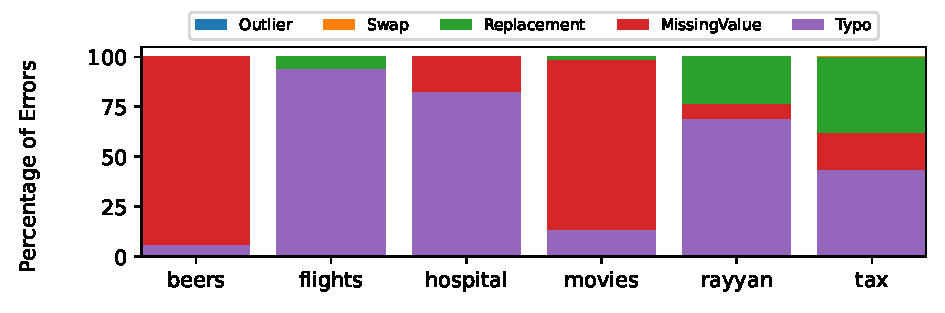
\includegraphics[width=\textwidth]{figures/plot/error_percent/errors_percent.pdf}
    \caption{Percentage of errors}
    \label{exp:errors_percent}
\end{figure}

\begin{figure}[!t]
    \centering
    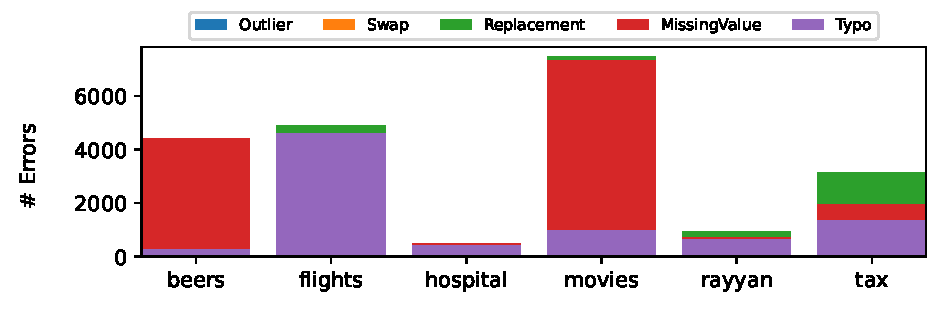
\includegraphics[width=\textwidth]{figures/plot/error_percent/errors.pdf}
    \caption{Frequency of errors}
    \label{exp:errors_count}
\end{figure}

\begin{table}[!t]
\centering
\caption{\label{tab:dirty_num_errors}Dirty Dataset Error Characteristics}
\begin{tabular}{r|K|K|K|K|K}
\toprule
                     & \colCenter{Outliers} & \colCenter{Typos} & \colCenter{MV}             & \colCenter{Replacements}              & \colCenterNoRight{Swaps}   \\ \midrule
beers                & \numprint{0}        & \numprint{254}   & \numprint{4170}           & \numprint{0}                & \numprint{0}       \\
flights              & \numprint{0}        & \numprint{4606}  & \numprint{0}              & \numprint{314}              & \numprint{0}       \\
hospital             & \numprint{0}        & \numprint{417}   & \numprint{92}             & \numprint{0}                & \numprint{0}       \\
movies               & \numprint{0}        & \numprint{982}  & \numprint{6346}           & \numprint{141}              & \numprint{0}       \\
rayyan               & \numprint{0}        & \numprint{649}   & \numprint{75}             & \numprint{224}              & \numprint{0}       \\
tax                  & \numprint{0}        & \numprint{1367}  & \numprint{588}            & \numprint{1200}             & \numprint{4}       \\ \bottomrule
\end{tabular}
\end{table}

\textbf{Distinct values:} 
Distinct values are also interesting in terms of data distribution, and errors impact the distinct items set.
Figure~\ref{exp:distinct_values_datasets} shows how the distinct value set in columns changes after error introduction. 
The x-axis represents each feature of the dataset, while the y-axis is log-scaled and shows the number of distinct values. 
The blue color represents clean data while the red color stands for dirty.
It is noticeable that in \textit{beers}, as stated earlier, one column is treated as completely missing.
On the other hand, in \textit{hospitals} and \textit{flights} the number of distinct items increases.
This happens because of many typos in both datasets.

\begin{figure}[!t]
    \centering 
    \centering
\begin{subfigure}{0.32\textwidth}
    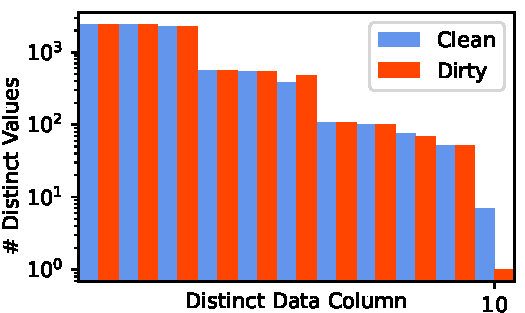
\includegraphics[width=\textwidth]{figures/plot/distinct/beers_distinct/combined.pdf}
    \caption{\label{exp:d1}Bears}
    \label{exp:distincts_bears}
\end{subfigure}
\hfill
\begin{subfigure}{0.32\textwidth}
    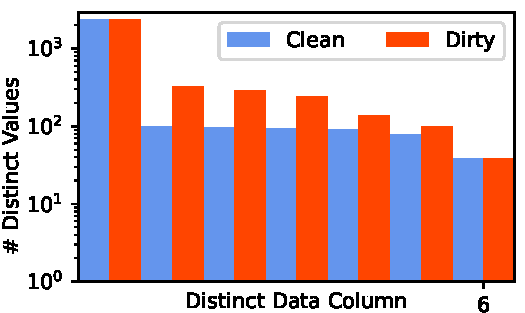
\includegraphics[width=\textwidth]{figures/plot/distinct/flights_distinct/combined.pdf}
    \caption{Flights}
    \label{exp:distincts_flights}
\end{subfigure}
\hfill
\begin{subfigure}{0.32\textwidth}
    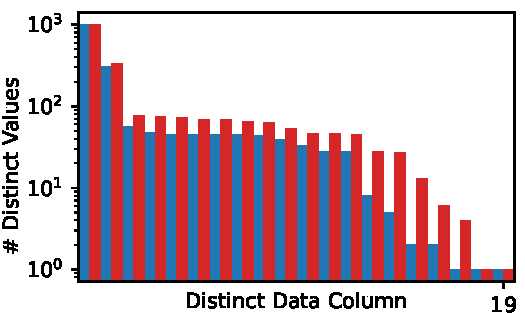
\includegraphics[width=\textwidth]{figures/plot/distinct/hospital_distinct/combined.pdf}
    \caption{Hospital}
    \label{fig:distincts_hospitals}
\end{subfigure}
\hfill
\begin{subfigure}{0.32\textwidth}
    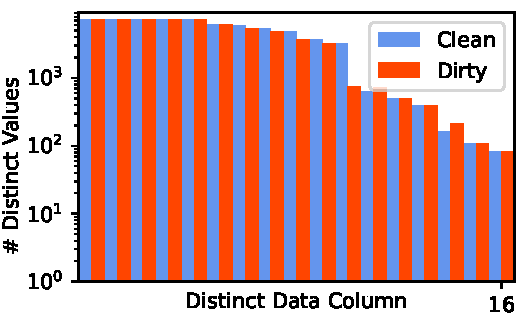
\includegraphics[width=\textwidth]{figures/plot/distinct/movies_distinct/combined.pdf}
    \caption{Movies}
    \label{exp:distincts_movies}
\end{subfigure}
\hfill
\begin{subfigure}{0.32\textwidth}
    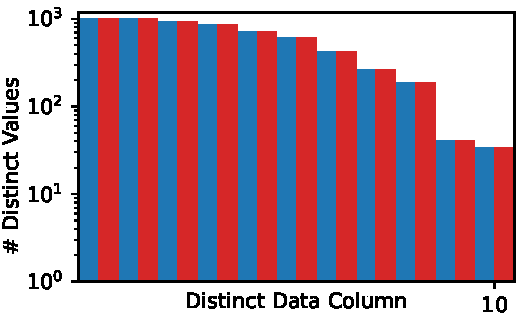
\includegraphics[width=\textwidth]{figures/plot/distinct/rayyan_distinct/combined.pdf}
    \caption{Rayyan}
    \label{exp:distincts_rayyan}
\end{subfigure}
\hfill
\begin{subfigure}{0.32\textwidth}
    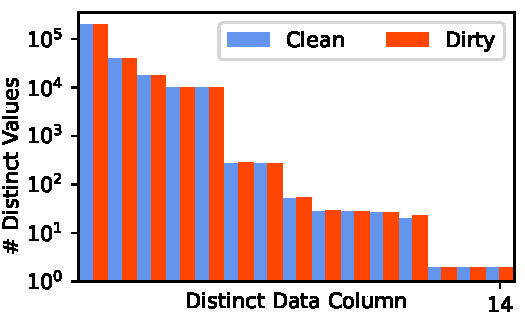
\includegraphics[width=\textwidth]{figures/plot/distinct/tax_distinct/combined.pdf}
    \caption{Tax}
    \label{exp:distincts_tax}
\end{subfigure}
\hfill
\caption{Distinct values distribution of clean and dirty datasets}
\label{exp:distinct_values_datasets}
\end{figure}

\newcolumntype{P}{>{\raggedleft\arraybackslash$}p{1.9cm}<{$}}
\newcolumntype{D}{>{\raggedleft\arraybackslash$}p{1.1cm}<{$}}

\begin{table}[!ht]
\caption{\label{tab:local_errors_beers} Local error distribution in beers}
\centering
\begin{tabular}{r|K|K|P|D|K}
\toprule
\colCenter{Scale} & \colCenter{Outliers} & \colCenter{Typos} & \colCenter{MV} & \colCenter{Replacements} & \colCenterNoRight{Swaps} \\ \midrule
\numprint{1}    & \numprint{0}        & \numprint{254}          & \numprint{4170}                 &  \numprint{0}     &  \numprint{0}              \\
\numprint{2}    & \numprint{0}        & \numprint{508}          & \numprint{8340}                 &  \numprint{0}     &  \numprint{0}              \\
\numprint{4}    & \numprint{0}        & \numprint{101}          & \numprint{16680}                 &  \numprint{0}     &  \numprint{0}              \\
\numprint{8}    & \numprint{0}        & \numprint{203}          & \numprint{33360}                 &  \numprint{0}     &  \numprint{0}              \\
\numprint{16}   & \numprint{0}        & \numprint{406}          & \numprint{66720}                 &  \numprint{0}     &  \numprint{0}              \\
\numprint{32}   & \numprint{0}        & \numprint{812}          & \numprint{133440}                 &  \numprint{0}     &  \numprint{0}              \\
\numprint{64}   & \numprint{0}        & \numprint{162}          & \numprint{266880}                 &  \numprint{0}     &  \numprint{0}              \\
\numprint{128}  & \numprint{0}        & \numprint{325}          & \numprint{533760}                 &  \numprint{0}     &  \numprint{0}              \\
\numprint{256}  & \numprint{0}        & \numprint{650}          & \numprint{1067520}                 &  \numprint{0}     &  \numprint{0}              \\
\bottomrule
\end{tabular}
\end{table}

\begin{table}[!ht]
\caption{\label{tab:local_errors_flights} Local error distribution in flights}
\centering
\begin{tabular}{r|K|P|D|K|K}
\toprule
\colCenter{Scale} & \colCenter{Outliers} & \colCenter{Typos} & \colCenter{MV} & \colCenter{Rep} & \colCenterNoRight{Swaps}  \\ \midrule
\numprint{1}             & \numprint{0}        & \numprint{4606}    & \numprint{0}             &  \numprint{314}  &  \numprint{0}              \\
\numprint{2}             & \numprint{0}        & \numprint{9212}    & \numprint{0}             &  \numprint{628}  &  \numprint{0}              \\
\numprint{4}             & \numprint{0}        & \numprint{18424}          & \numprint{0}             &  \numprint{1256}     &  \numprint{0}              \\
\numprint{8}             & \numprint{0}        & \numprint{36848}          & \numprint{0}             &  \numprint{2512}     &  \numprint{0}              \\
\numprint{16}             & \numprint{0}        & \numprint{73696}          & \numprint{0}             &  \numprint{5024}     &  \numprint{0}              \\
\numprint{32}             & \numprint{0}        & \numprint{147392}          & \numprint{0}             &  \numprint{10048}     &  \numprint{0}              \\
\numprint{64}             & \numprint{0}        & \numprint{294784}          & \numprint{0}             &  \numprint{20096}     &  \numprint{0}              \\
\numprint{128} & \numprint{0} & \numprint{589568}  & \numprint{0} & \numprint{40192} & \numprint{0} \\
\numprint{256} & \numprint{0} & \numprint{1179136} & \numprint{0} & \numprint{80384} & \numprint{0} \\
\bottomrule
\end{tabular}
\end{table}

\begin{table}[!ht]
\caption{\label{tab:local_errors_hospital} Local error distribution in hospital}
\centering
\begin{tabular}{r|K|K|K|K|K}
\toprule
\colCenter{Scale} & \colCenter{Outliers} & \colCenter{Typos} & \colCenter{MV} & \colCenter{Rep} & \colCenterNoRight{Swaps}  \\ \midrule
\numprint{1}        & \numprint{0}        & \numprint{417}         & \numprint{92}                &  \numprint{0}       &  \numprint{0}     \\
\numprint{2}        & \numprint{0}        & \numprint{834}         & \numprint{184}               &  \numprint{0}       &  \numprint{0}     \\
\numprint{4}        & \numprint{0}        & \numprint{1668}        & \numprint{368}               &  \numprint{0}       &  \numprint{0}     \\
\numprint{8}        & \numprint{0}        & \numprint{3336}        & \numprint{736}               &  \numprint{0}       &  \numprint{0}     \\
\numprint{16}       & \numprint{0}        & \numprint{6672}        & \numprint{1472}              &  \numprint{0}       &  \numprint{0}     \\
\numprint{32}       & \numprint{0}        & \numprint{13344}       & \numprint{2944}              &  \numprint{0}       &  \numprint{0}     \\
\numprint{64}       & \numprint{0}        & \numprint{26688}       & \numprint{5888}              &  \numprint{0}       &  \numprint{0}     \\ 
\numprint{128}      & \numprint{0}        & \numprint{53376}       & \numprint{11776}             &  \numprint{0}       &  \numprint{0}     \\
\numprint{256}      & \numprint{0}        & \numprint{106752}      & \numprint{23552}             &  \numprint{0}       &  \numprint{0}     \\
\bottomrule
\end{tabular}
\end{table}

\begin{table}[!ht]
\caption{\label{tab:local_errors_movies} Local error distribution in movies}
\centering
\begin{tabular}{r|K|K|P|K|K}
\toprule
\colCenter{Scale} & \colCenter{Outliers} & \colCenter{Typos} & \colCenter{MV} & \colCenter{Rep} & \colCenterNoRight{Swaps}  \\ \midrule
\numprint{1}        & \numprint{0}        & \numprint{982}      & \numprint{6346}       &  \numprint{142}   &  \numprint{0}       \\
\numprint{2}        & \numprint{0}        & \numprint{1964}     & \numprint{12692}      &  \numprint{284}   &  \numprint{0}       \\
\numprint{4}        & \numprint{0}        & \numprint{3928}     & \numprint{25384}      &  \numprint{568}   &  \numprint{0}       \\
\numprint{8}        & \numprint{0}        & \numprint{7856}     & \numprint{50768}      &  \numprint{1136}  &  \numprint{0}       \\
\numprint{16}       & \numprint{0}        & \numprint{15712}    & \numprint{101536}     &  \numprint{2272}  &  \numprint{0}       \\
\numprint{32}       & \numprint{0}        & \numprint{31424}    & \numprint{203072}     &  \numprint{4544}  &  \numprint{0}       \\
\numprint{64}       & \numprint{0}        & \numprint{62848}    & \numprint{406144}     &  \numprint{9088}  &  \numprint{0}       \\
\numprint{128}      & \numprint{0}        & \numprint{125696}   & \numprint{812288}     &  \numprint{18176} &  \numprint{0}       \\ 
\numprint{256}      & \numprint{0}        & \numprint{251392}   & \numprint{1624576}    &  \numprint{36352} &  \numprint{0}       \\   \bottomrule
\end{tabular}
\end{table}

\begin{table}[!ht]
\caption{\label{tab:local_errors_rayyan} Local error distribution in rayyan}
\centering
\begin{tabular}{r|K|K|K|K|K}
\toprule
\colCenter{Scale} & \colCenter{Outliers} & \colCenter{Typos} & \colCenter{MV} & \colCenter{Rep} & \colCenterNoRight{Swaps}  \\ \midrule
\numprint{1}         & \numprint{0}        & \numprint{649}       & \numprint{75}       &  \numprint{224}       &  \numprint{0}              \\
\numprint{2}         & \numprint{0}        & \numprint{1298}      & \numprint{150}      &  \numprint{448}       &  \numprint{0}              \\
\numprint{4}         & \numprint{0}        & \numprint{2596}      & \numprint{300}      &  \numprint{896}       &  \numprint{0}              \\
\numprint{8}         & \numprint{0}        & \numprint{5192}      & \numprint{600}      &  \numprint{1792}      &  \numprint{0}              \\
\numprint{16}        & \numprint{0}        & \numprint{10384}     & \numprint{1200}     &  \numprint{3584}      &  \numprint{0}              \\
\numprint{32}        & \numprint{0}        & \numprint{20768}     & \numprint{2400}     &  \numprint{7168}      &  \numprint{0}              \\
\numprint{64}        & \numprint{0}        & \numprint{41536}     & \numprint{4800}     &  \numprint{14336}     &  \numprint{0}              \\ 
\numprint{128}       & \numprint{0}        & \numprint{83072}     & \numprint{9600}     &  \numprint{28672}     &  \numprint{0}              \\ 
\numprint{256}       & \numprint{0}        & \numprint{166144}    & \numprint{19200}    &  \numprint{57344}     &  \numprint{0}              \\  \bottomrule
\end{tabular}
\end{table}

\textbf{Scaled error distribution:} 
Table~\ref{tab:local_errors_tax} shows the scaled error distribution for the \textit{tax} dataset.
In the Table row 1 is the error distribution of original dirty data.
It is guaranteed that errors scale linearly within 10\% of original number of errors.
It can be observed that there is no necessity in 10\% bound for local execution since number of errors is perfectly matching the expected. 
% TODO compare to distributed
Other datasets are described in Table~\ref{tab:local_errors_beers} - \textit{beers}, Table~\ref{tab:local_errors_hospital} - \textit{hospital},
Table~\ref{tab:local_errors_flights} - \textit{flights}, Table~\ref{tab:local_errors_beers} -  \textit{movies}, and Table~\ref{tab:local_errors_rayyan} - \textit{rayyan}. 


\begin{table}[!t]
\caption{\label{tab:local_errors_tax} Local error distribution in tax}
\centering
\begin{tabular}{r|K|K|K|K|K}
\toprule
\colCenter{Scale} & \colCenter{Outliers} & \colCenter{Typos} & \colCenter{MV} & \colCenter{Rep} & \colCenterNoRight{Swaps}  \\ \midrule
 \numprint{1}  &   \numprint{2} &   \numprint{1367} &    \numprint{588} &    \numprint{1200} &    \numprint{4} \\
 \numprint{2}  &   \numprint{4} &   \numprint{2734} &   \numprint{1176} &    \numprint{2400} &    \numprint{8} \\
 \numprint{4}  &   \numprint{8} &   \numprint{5468} &   \numprint{2352} &    \numprint{4800} &   \numprint{16} \\
 \numprint{8}  &  \numprint{16} &  \numprint{10936} &   \numprint{4704} &    \numprint{9600} &   \numprint{32} \\
\numprint{16}  &  \numprint{32} &  \numprint{21842} &   \numprint{9408} &   \numprint{19200} &   \numprint{64} \\
\numprint{32}  &  \numprint{64} &  \numprint{43744} &  \numprint{18816} &   \numprint{38400} &  \numprint{128} \\
\numprint{64}  & \numprint{128} &  \numprint{87488} &  \numprint{37632} &   \numprint{76800} &  \numprint{256} \\
\numprint{128} & \numprint{256} & \numprint{174976} &  \numprint{75264} &  \numprint{153600} &  \numprint{512} \\
\numprint{256} & \numprint{512} & \numprint{349952} & \numprint{150528} &  \numprint{307200} & \numprint{1024} \\
\bottomrule
\end{tabular}
\end{table}

\textbf{Distinct values:} 
Scaling distinct values is more challenging. 
Table~\ref{tab:dist_errors_tax} shows how the number of distinct values of each error type changes for different scaling factors.
Typos, missing values and distincts are represented by estimated (\textit{Est}) and actual (\textit{Act}) number of distinct items.
It is noticeable that typos are scaled according to the estimation.
Missing values differ from estimation because the set of new distinct missing values, that can be added randomly, is limited. % and hard-coded.
There is no estimation of distinct outlier values since the original outlier distribution is fully reused, and newly generated values are used instead of original. 
Column \textit{Distinct} represents number of estimated and observed number of distinct values in the whole dataset.
Since some errors are introduced at random, it is expected that estimation slightly differs from actual value. 

\newcolumntype{S}{>{\raggedleft\arraybackslash$}p{2.0cm}<{$}}

\begin{table}[!ht]
\caption{\label{tab:dist_errors_beer} Local errors distincts in beer}
\centering
\begin{tabular}{r|K|K|H|H||K|K}
\toprule
               & \multicolumn{2}{c|}{\textbf{Typos}}   & \multicolumn{2}{c||}{\textbf{MV}}  & \multicolumn{2}{c}{\textbf{Distinct}}\\
\colCenter{Scale} & \colCenter{Est} & \colCenter{Act} & \colCenter{Est} & \multicolumn{1}{c||}{\textbf{{Act}}} & \colCenter{Est}   & \colCenterNoRight{Act}   \\ \midrule
\numprint{1}          &  \numprint{97}      & \numprint{97}          & \numprint{3}  & \numprint{6}  & \numprint{9038}  & \numprint{9038}     \\
\numprint{2}          &  \numprint{167}     & \numprint{167}         & \numprint{3}  & \numprint{6}  & \numprint{9128}  & \numprint{9116}     \\
\numprint{4}          &  \numprint{290}     & \numprint{290}         & \numprint{3}  & \numprint{6}  & \numprint{9251}  & \numprint{9241}     \\
\numprint{8}          &  \numprint{526}     & \numprint{526}         & \numprint{3}  & \numprint{6}  & \numprint{9487}  & \numprint{9474}     \\
\numprint{16}         &  \numprint{994}     & \numprint{994}         & \numprint{3}  & \numprint{6}  & \numprint{9955}  & \numprint{9938}     \\
\numprint{32}         &  \numprint{1926}    & \numprint{1923}        & \numprint{3}  & \numprint{6}  & \numprint{10887}  & \numprint{10866}     \\
\numprint{64}         &  \numprint{3789}    & \numprint{3786}        & \numprint{3}  & \numprint{6}  & \numprint{12750}  & \numprint{12699}     \\ 
\numprint{128}        &  \numprint{7514}    & \numprint{7405}        & \numprint{3}  & \numprint{6}  & \numprint{16475}  & \numprint{16290}     \\
\numprint{256}        &  \numprint{14964}   & \numprint{14575}       & \numprint{3}  & \numprint{6}  & \numprint{23925}  & \numprint{23420}     \\
\bottomrule
\end{tabular}
\end{table}

\begin{table}[!ht]
\caption{\label{tab:dist_errors_flights} Local errors distincts in flights}
\centering
\begin{tabular}{r|K|K|H|H||K|K}
\toprule
               & \multicolumn{2}{c|}{\textbf{Typos}}   & \multicolumn{2}{c||}{\textbf{MV}}  & \multicolumn{2}{c}{\textbf{Distinct}}\\
\colCenter{Scale} & \colCenter{Est} & \colCenter{Act} & \colCenter{Est} & \multicolumn{1}{c||}{\textbf{{Act}}} & \colCenter{Est}   & \colCenterNoRight{Act}   \\ \midrule
\numprint{1}         & \numprint{651}   & \numprint{651}    & \numprint{0}  & \numprint{0}  & \numprint{3512}   & \numprint{3512}    \\
\numprint{2}         & \numprint{808}   & \numprint{808}    & \numprint{0}  & \numprint{0}  & \numprint{3682}   & \numprint{3682}    \\
\numprint{4}         & \numprint{1012}  & \numprint{1012}   & \numprint{0}  & \numprint{0}  & \numprint{3886}   & \numprint{3883}    \\
\numprint{8}         & \numprint{1334}  & \numprint{1334}   & \numprint{0}  & \numprint{0}  & \numprint{4208}   & \numprint{4204}    \\
\numprint{16}        & \numprint{1940}  & \numprint{1937}   & \numprint{0}  & \numprint{0}  & \numprint{4814}   & \numprint{4796}    \\
\numprint{32}        & \numprint{3136}  & \numprint{3126}   & \numprint{0}  & \numprint{0}  & \numprint{6010}   & \numprint{5974}    \\
\numprint{64}        & \numprint{5521}  & \numprint{5473}   & \numprint{0}  & \numprint{0}  & \numprint{8395}   & \numprint{8309}    \\
\numprint{128}       & \numprint{10151} & \numprint{10012}  & \numprint{0}  & \numprint{0}  & \numprint{13025}  & \numprint{12816}     \\
\numprint{256}       & \numprint{17301} & \numprint{16968}  & \numprint{0}  & \numprint{0}  & \numprint{20175}  & \numprint{19728}     \\
\bottomrule
\end{tabular}
\end{table}

\begin{table}[!ht]
\caption{\label{tab:dist_errors_hospital} Local errors distincts in hospital}
\centering
\begin{tabular}{r|K|K|H|H||K|K}
\toprule
               & \multicolumn{2}{c|}{\textbf{Typos}}   & \multicolumn{2}{c||}{\textbf{MV}}  & \multicolumn{2}{c}{\textbf{Distinct}}\\
\colCenter{Scale} & \colCenter{Est} & \colCenter{Act} & \colCenter{Est} & \multicolumn{1}{c||}{\textbf{{Act}}} & \colCenter{Est}   & \colCenterNoRight{Act}   \\ \midrule
\numprint{1}         & \numprint{311}   & \numprint{311}  & \numprint{3}  & \numprint{3}  & \numprint{2094} & \numprint{2094}    \\
\numprint{2}         & \numprint{568}   & \numprint{568}  & \numprint{3}  & \numprint{6}  & \numprint{2357} & \numprint{2355}    \\
\numprint{4}         & \numprint{1060}  & \numprint{1058}  & \numprint{3}  & \numprint{6}  & \numprint{2849} & \numprint{2841}    \\
\numprint{8}         & \numprint{2039}  & \numprint{2037}  & \numprint{3}  & \numprint{6}  & \numprint{3828} & \numprint{3809}    \\
\numprint{16}        & \numprint{3992}  & \numprint{3977}  & \numprint{3}  & \numprint{6}  & \numprint{5781} & \numprint{5735}    \\
\numprint{32}        & \numprint{7899}  & \numprint{7839}  & \numprint{3}  & \numprint{6}  & \numprint{9688} & \numprint{9571}    \\
\numprint{64}        & \numprint{15711} & \numprint{15493}  & \numprint{3}  & \numprint{6}  & \numprint{17200} & \numprint{17181}     \\ 
\numprint{128}       & \numprint{31336} & \numprint{30223}  & \numprint{3}  & \numprint{6}  & \numprint{33125} & \numprint{31801}     \\ 
\numprint{256}       & \numprint{62584} & \numprint{59268}  & \numprint{3}  & \numprint{6}  & \numprint{64373} & \numprint{60722}     \\ 
\bottomrule
\end{tabular}
\end{table}

\begin{table}[!ht]
\caption{\label{tab:dist_errors_movies} Local errors distincts in movies}
\centering
\begin{tabular}{r|K|K|H|H||K|K}
\toprule
               & \multicolumn{2}{c|}{\textbf{Typos}}   & \multicolumn{2}{c||}{\textbf{MV}}  & \multicolumn{2}{c}{\textbf{Distinct}}\\
\colCenter{Scale} & \colCenter{Est} & \colCenter{Act} & \colCenter{Est} & \multicolumn{1}{c||}{\textbf{{Act}}} & \colCenter{Est}   & \colCenterNoRight{Act}   \\ \midrule
\numprint{1}        & \numprint{868}    & \numprint{868}    & \numprint{3}  & \numprint{3}  & \numprint{62444}  & \numprint{62444}    \\
\numprint{2}        & \numprint{1667}   & \numprint{1667}   & \numprint{3}  & \numprint{6}  & \numprint{69010}  & \numprint{68659}    \\
\numprint{4}        & \numprint{3227}   & \numprint{3226}   & \numprint{3}  & \numprint{6}  & \numprint{70570}  & \numprint{68547}    \\
\numprint{8}        & \numprint{6321}   & \numprint{6317}   & \numprint{3}  & \numprint{6}  & \numprint{73664}  & \numprint{72970}    \\
\numprint{16}       & \numprint{12498}  & \numprint{12494}  & \numprint{3}  & \numprint{6}  & \numprint{79841}  & \numprint{79702}    \\
\numprint{32}       & \numprint{24846}  & \numprint{24833}  & \numprint{3}  & \numprint{6}  & \numprint{92189}  & \numprint{92066}    \\
\numprint{64}       & \numprint{49539}  & \numprint{49486}  & \numprint{3}  & \numprint{6}  & \numprint{116882} & \numprint{116613}     \\ 
\numprint{128}      & \numprint{98924}  & \numprint{98746}  & \numprint{3}  & \numprint{6}  & \numprint{166267} & \numprint{165632}     \\ 
\numprint{256}      & \numprint{197695} & \numprint{197100} & \numprint{3}  & \numprint{6}  & \numprint{265038} & \numprint{263634}     \\ 

\bottomrule
\end{tabular}
\end{table}

\begin{table}[!t]
\caption{\label{tab:dist_errors_tax} Local errors distincts in tax}
\centering
\begin{tabular}{r|H|H|H|H|K||K|S}
\toprule
               & \multicolumn{2}{c|}{\textbf{Typos}}   & \multicolumn{2}{c|}{\textbf{MV}} &   \multicolumn{1}{c||}{\textbf{Outliers}} &  \multicolumn{2}{c}{\textbf{Distinct}}\\
\colCenter{Scale} & \colCenter{Est} & \colCenter{Act} &  \colCenter{Est} & \colCenter{Act} & \multicolumn{1}{c||}{\textbf{{Act}}} & \colCenter{Est}   & \colCenterNoRight{Act}   \\ \midrule
\numprint{1}              & \numprint{81}  & \numprint{81}    & \numprint{6}    & \numprint{6}    &  \numprint{2}  & \numprint{275201}   & \numprint{275201}   \\
\numprint{2}              & \numprint{83}  & \numprint{83}    & \numprint{9}    & \numprint{11}   &  \numprint{4}  & \numprint{275260}   & \numprint{275257}   \\
\numprint{4}              & \numprint{84}  & \numprint{84}    & \numprint{15}   & \numprint{16}   &  \numprint{4}  & \numprint{275271}   & \numprint{275261}   \\
\numprint{8}              & \numprint{86}  & \numprint{86}    & \numprint{27}   & \numprint{22}   &  \numprint{5}  & \numprint{275293}   & \numprint{275272}   \\
\numprint{16}             & \numprint{89}  & \numprint{89}    & \numprint{51}   & \numprint{28}   &  \numprint{5}  & \numprint{275336}   & \numprint{275286}   \\
\numprint{32}             & \numprint{96}  & \numprint{96}    & \numprint{89}   & \numprint{29}   &  \numprint{8}  & \numprint{275413}   & \numprint{275296}   \\
\numprint{64}             & \numprint{107} & \numprint{107}   & \numprint{138}  & \numprint{23}   &  \numprint{12} & \numprint{275537}   & \numprint{275306}   \\ 
\numprint{128}            & \numprint{129} & \numprint{129}   & \numprint{264}  & \numprint{22}   &  \numprint{32} & \numprint{275813}   & \numprint{275332}   \\
\bottomrule
\end{tabular}
\end{table}


\begin{figure}[!t]
    \centering 
    \centering
\begin{subfigure}{0.32\textwidth}
    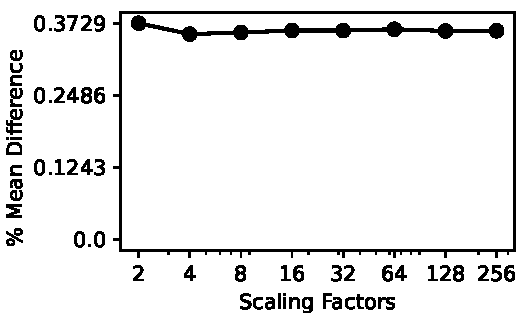
\includegraphics[width=\textwidth]{figures/plot/mean/mean_diff_beers.pdf}
    \caption{Bears}
    \label{exp:mean_bears}
\end{subfigure}
\hfill
\begin{subfigure}{0.32\textwidth}
    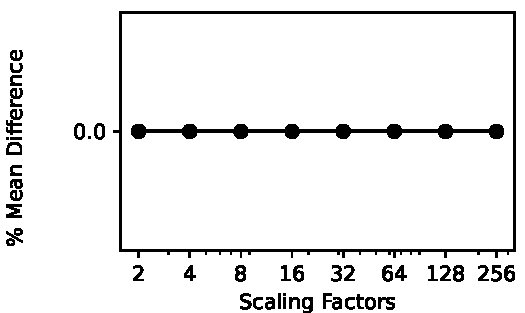
\includegraphics[width=\textwidth]{figures/plot/mean/mean_diff_flights.pdf}
    \caption{Flights}
    \label{exp:mean_flights}
\end{subfigure}
\hfill
\begin{subfigure}{0.32\textwidth}
    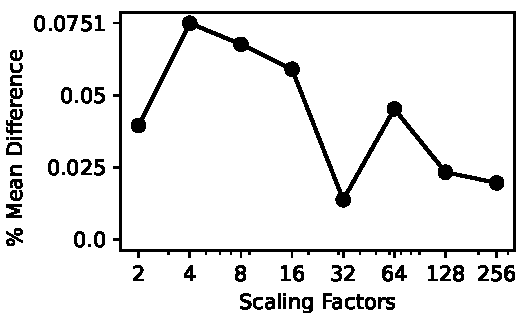
\includegraphics[width=\textwidth]{figures/plot/mean/mean_diff_hospital.pdf}
    \caption{Hospital}
    \label{fig:mean_hospitals}
\end{subfigure}
\hfill
\begin{subfigure}{0.32\textwidth}
    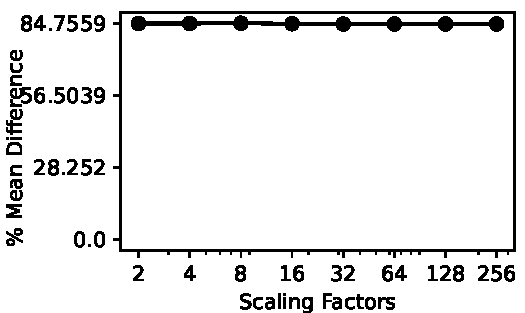
\includegraphics[width=\textwidth]{figures/plot/mean/mean_diff_movies.pdf}
    \caption{Movies}
    \label{exp:mean_movies}
\end{subfigure}
\hfill
\begin{subfigure}{0.32\textwidth}
    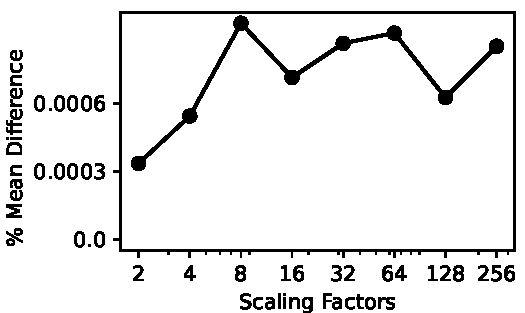
\includegraphics[width=\textwidth]{figures/plot/mean/mean_diff_rayyan.pdf}
    \caption{Rayyan}
    \label{exp:mean_rayyan}
\end{subfigure}
\hfill
\begin{subfigure}{0.32\textwidth}
    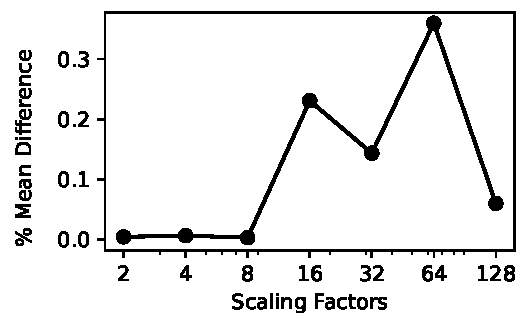
\includegraphics[width=\textwidth]{figures/plot/mean/mean_diff_tax.pdf}
    \caption{Tax}
    \label{exp:mean_tax}
\end{subfigure}
\hfill
\caption{Mean difference in percent scaling clean and dirty datasets}
\label{exp:mean_difference_datasets}
\end{figure}


\begin{figure}[!t]
    \centering 
    \centering
\begin{subfigure}{0.32\textwidth}
    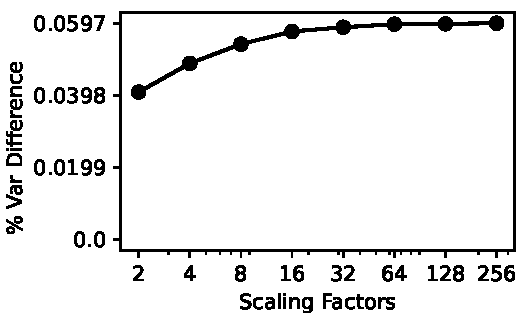
\includegraphics[width=\textwidth]{figures/plot/var/variance_diff_beers.pdf}
    \caption{Bears}
    \label{exp:var_bears}
\end{subfigure}
\hfill
\begin{subfigure}{0.32\textwidth}
    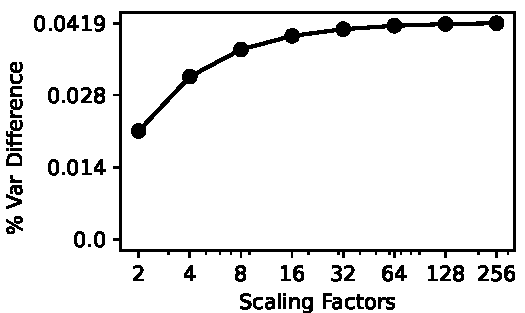
\includegraphics[width=\textwidth]{figures/plot/var/variance_diff_flights.pdf}
    \caption{Flights}
    \label{exp:var_flights}
\end{subfigure}
\hfill
\begin{subfigure}{0.32\textwidth}
    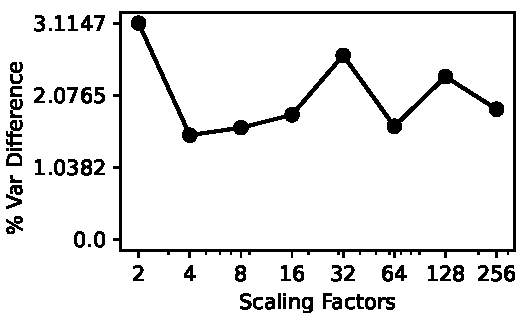
\includegraphics[width=\textwidth]{figures/plot/var/variance_diff_hospital.pdf}
    \caption{Hospital}
    \label{fig:var_hospitals}
\end{subfigure}
\hfill
\begin{subfigure}{0.32\textwidth}
    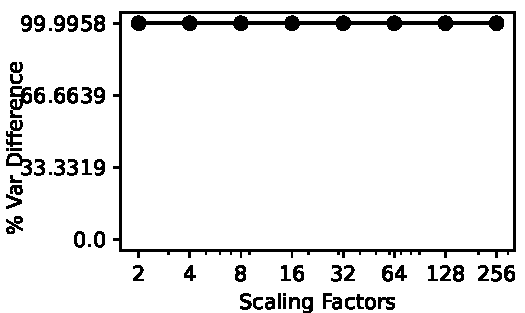
\includegraphics[width=\textwidth]{figures/plot/var/variance_diff_movies.pdf}
    \caption{Movies}
    \label{exp:var_movies}
\end{subfigure}
\hfill
\begin{subfigure}{0.32\textwidth}
    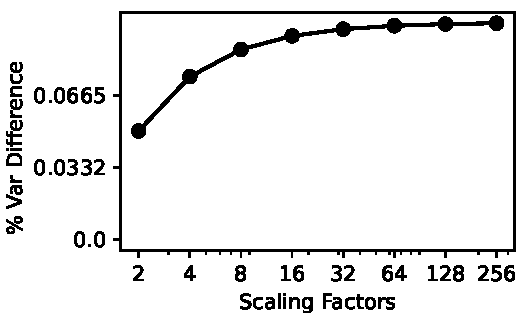
\includegraphics[width=\textwidth]{figures/plot/var/variance_diff_rayyan.pdf}
    \caption{Rayyan}
    \label{exp:var_rayyan}
\end{subfigure}
\hfill
\begin{subfigure}{0.32\textwidth}
    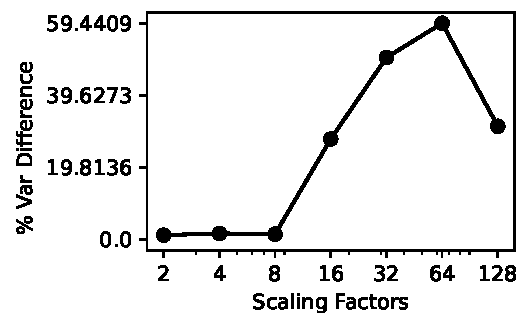
\includegraphics[width=\textwidth]{figures/plot/var/variance_diff_tax.pdf}
    \caption{Tax}
    \label{exp:var_tax}
\end{subfigure}
\hfill
\caption{Variance difference in percent scaling clean and dirty datasets}
\label{exp:var_difference_datasets}
\end{figure}

\begin{figure}[!ht]
    \centering 
    \centering
\begin{subfigure}{0.32\textwidth}
    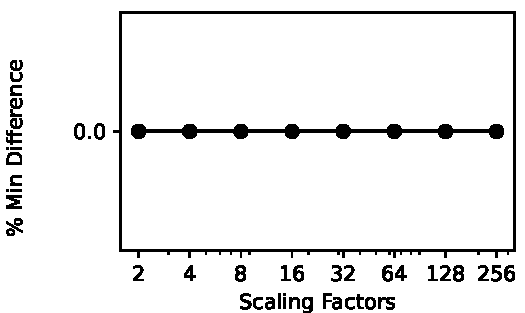
\includegraphics[width=\textwidth]{figures/plot/min/min_diff_beers.pdf}
    \caption{Bears}
    \label{exp:min_bears}
\end{subfigure}
\hfill
\begin{subfigure}{0.32\textwidth}
    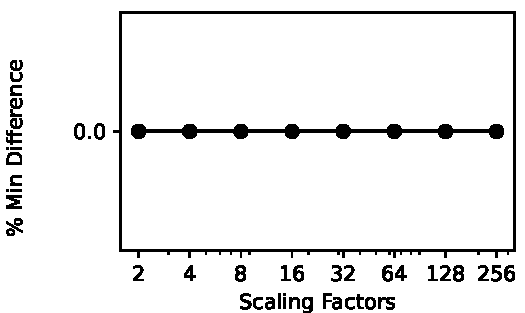
\includegraphics[width=\textwidth]{figures/plot/min/min_diff_flights.pdf}
    \caption{Flights}
    \label{exp:min_flights}
\end{subfigure}
\hfill
\begin{subfigure}{0.32\textwidth}
    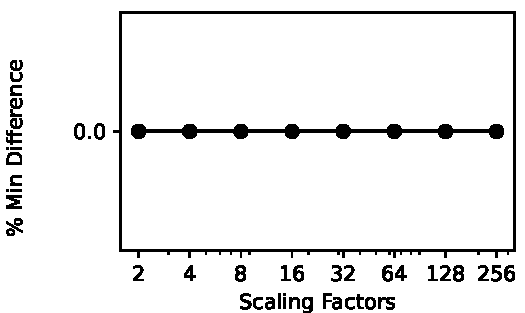
\includegraphics[width=\textwidth]{figures/plot/min/min_diff_hospital.pdf}
    \caption{Hospital}
    \label{fig:min_hospitals}
\end{subfigure}
\hfill
\begin{subfigure}{0.32\textwidth}
    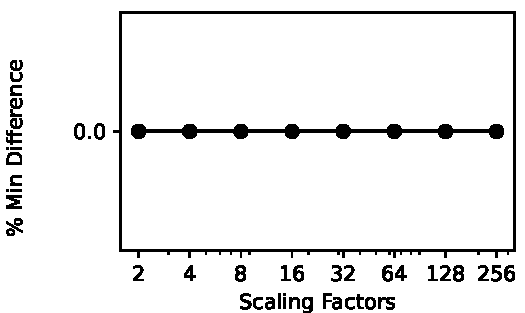
\includegraphics[width=\textwidth]{figures/plot/min/min_diff_movies.pdf}
    \caption{Movies}
    \label{exp:min_movies}
\end{subfigure}
\hfill
\begin{subfigure}{0.32\textwidth}
    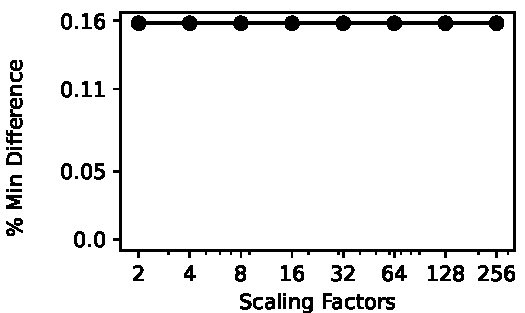
\includegraphics[width=\textwidth]{figures/plot/min/min_diff_rayyan.pdf}
    \caption{Rayyan}
    \label{exp:min_rayyan}
\end{subfigure}
\hfill
\begin{subfigure}{0.32\textwidth}
    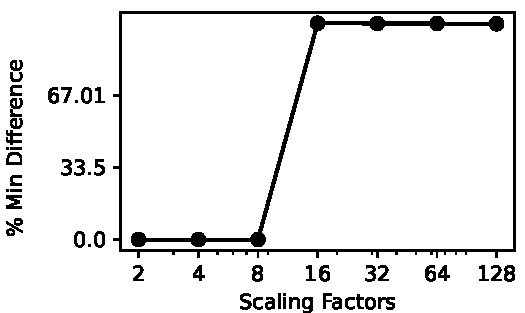
\includegraphics[width=\textwidth]{figures/plot/min/min_diff_tax.pdf}
    \caption{Tax}
    \label{exp:min_tax}
\end{subfigure}
\hfill
\caption{Min value difference in percent scaling clean and dirty datasets}
\label{exp:min_difference_datasets}
\end{figure}

\begin{figure}[!ht]
    \centering 
    \centering
\begin{subfigure}{0.32\textwidth}
    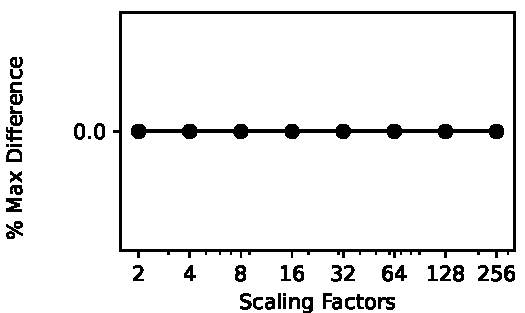
\includegraphics[width=\textwidth]{figures/plot/max/max_diff_beers.pdf}
    \caption{Bears}
    \label{exp:max_bears}
\end{subfigure}
\hfill
\begin{subfigure}{0.32\textwidth}
    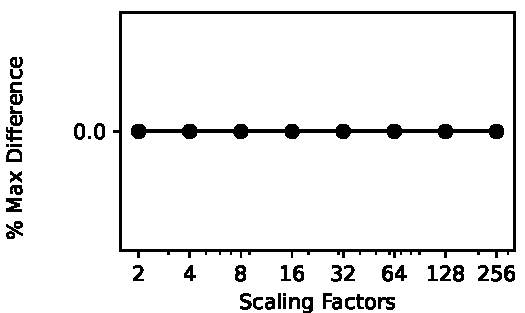
\includegraphics[width=\textwidth]{figures/plot/max/max_diff_flights.pdf}
    \caption{Flights}
    \label{exp:max_flights}
\end{subfigure}
\hfill
\begin{subfigure}{0.32\textwidth}
    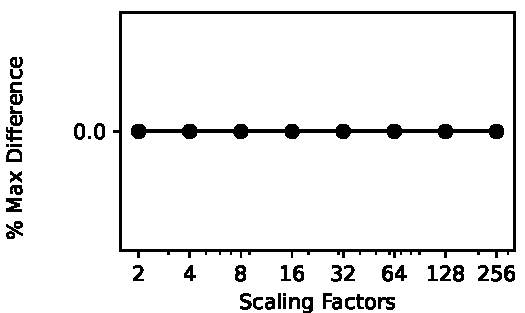
\includegraphics[width=\textwidth]{figures/plot/max/max_diff_hospital.pdf}
    \caption{Hospital}
    \label{fig:max_hospitals}
\end{subfigure}
\hfill
\begin{subfigure}{0.32\textwidth}
    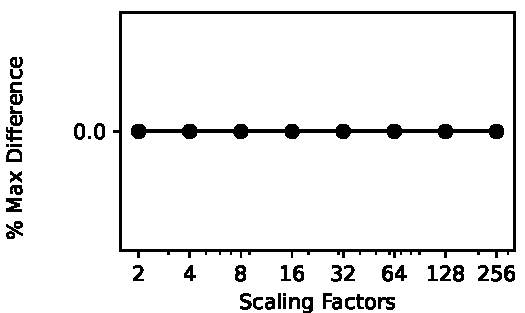
\includegraphics[width=\textwidth]{figures/plot/max/max_diff_movies.pdf}
    \caption{Movies}
    \label{exp:max_movies}
\end{subfigure}
\hfill
\begin{subfigure}{0.32\textwidth}
    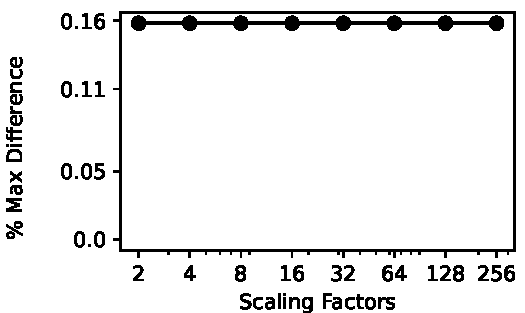
\includegraphics[width=\textwidth]{figures/plot/max/max_diff_rayyan.pdf}
    \caption{Rayyan}
    \label{exp:max_rayyan}
\end{subfigure}
\hfill
\begin{subfigure}{0.32\textwidth}
    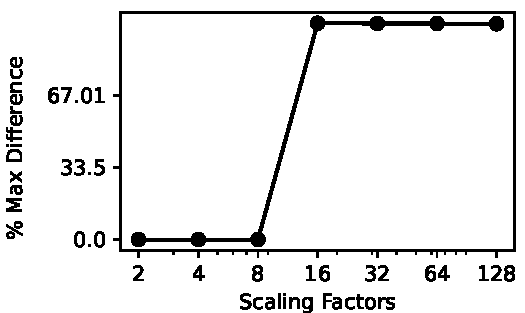
\includegraphics[width=\textwidth]{figures/plot/max/max_diff_tax.pdf}
    \caption{Tax}
    \label{exp:max_tax}
\end{subfigure}
\hfill
\caption{Max value difference in percent scaling clean and dirty datasets}
\label{exp:max_difference_datasets}
\end{figure}

\textbf{Statistics of generated dataset:} 
After generation, statistics are expected to be within 5\% of original statistics.
Figures~\ref{exp:mean_difference_datasets} and \ref{exp:var_difference_datasets} show that mean and variance are preserved.
In all figures, x-axis represents the scaling factor and y-axis is the percent difference of the original dirty and generated mean.
The percentage difference is less than 1\% for all datasets except \textit{movies}.
Since the \textit{movies} dataset contains one fully missing column, as mentioned before, and the statistical properties are not preserved, mean of the \textit{movies} is infinity. 
The \textit{tax} dataset variance also differs from the original variance because introduced outlier values are significantly different from the clean dataset distinct values.
The min and max plots are presented in Figure~\ref{exp:min_difference_datasets} and Figure~\ref{exp:max_difference_datasets} respectively.
All above mentioned data characteristics are preserved in both local and distributed data generators.
